% !TeX spellcheck = en_US
\addscenariosection{1}{Cooperative Scenario}{Close to Enemies}{\images/ballistics.png}

\begin{multicols}{2}

\textbf{Author:} Kelghor

\textit{``Sir! The raiders are at our gates!''}

\textit{``Sound the warhorn! We'll drive them back as always!'' you command, and go to defend the city. Just as you have done many times before. Such is the harsh life of the border clans, where wars and skirmishes with neighboring rivals never truly end. Fortunately, your alliance remains strong, and you know your back is covered.}

\textit{The time has come to end these long-standing wars and crush your enemies like a bug once and for all!}
% Translator info: In Homam IV was Quote like: "Rufux will crush this army like a bug." If has scounting and has bigger army. So "like a bug" is little easter egg referencing on this.

\subsection*{\MakeUppercase{Scenario Length}}

This Scenario is played over 7 Rounds.

\subsection*{\MakeUppercase{Player Setup}}

\textbf{Player Count:} 1--6

\textbf{Starting Resources:} 14 \svg{gold}, 5 \svg{building_materials}, 2 \svg{valuables}

\textbf{Starting Income:} 10 \svg{gold}, 2 \svg{building_materials}, 0 \svg{valuables}

\textbf{Starting Units:}
\begin{itemize}
  \item  1 × A Few \bronze\ Units of your choice
\end{itemize}

\textbf{Town Buildings:} \bronze\ Dwelling

\subsection*{\MakeUppercase{Map Setup}}

Take the following Map Tiles and arrange them as shown in the Scenario map layout ($P$ stands for the number of players):

\begin{itemize}
  \item P × Starting (I) Map Tile
  \item 4P × Far (II--III) Map Tile of the same terrain as player's Town, one of which must contain a Settlement
\end{itemize}

Place Far (II--III) Map Tiles with Settlements matching your Faction's terrain in positions marked by colored Cubes in the Scenario map layout.
Each pair of same-colored Cubes indicates a Starting (I) Map Tile and its corresponding Far (II--III) Map Tile with a Settlement.

\textbf{Map Tile Pool (choose one):}

\begin{itemize}
  \item \textbf{Personal Pool:} Each player takes remaining 1~×~Far (II--III) Map Tile without a Settlement that matches their Town's terrain
  \item \textbf{Shared Pool:}
  \begin{itemize}
    \item Remove all Far (II--III) Map Tiles without Settlements from the Map
    \item Take collected Map Tiles from the Map and remaining prepared Tiles and shuffle them together
    \item Return the shuffled Map Tiles to the Map in random order
    \item Remaining Map Tiles form the Shared Pool
  \end{itemize}
\end{itemize}

\subsection*{\MakeUppercase{AI Hero Setup}}

Prepare an AI Deck for Settlement defenders.

\textbf{Settlement defenders Deck:} 1 × Attack Card, 1 × Defense Card, 1 × Spell Card

\textbf{Settlement defenders Spell Deck:} 1~×~Magic Arrow

\subsection*{\MakeUppercase{Victory Conditions}}

\begin{itemize}
   \item Conquer all Settlements.
\end{itemize}

\subsection*{\MakeUppercase{Defeat Conditions}}

\begin{itemize}
  \item Any player loses their Town.
  \item At least one Settlement remains unclaimed by the end of the \nth{7} Round. Time has run out!
\end{itemize}

\subsection*{\MakeUppercase{Timed Events}}
\textbf{\nth{1} Round:}
\begin{itemize}
  \item At the start of the Round, all players reveal their \textit{Nemesis Map Tiles} (Far (II--III) Map Tiles containing Settlements that match their Town's home terrain). These Tiles may be revealed without any cost.
\end{itemize}
\textbf{\nth{2} Round:}
\begin{itemize}
  \item The first wave of Enemy Clan armies attacks all Towns (see section below).
  \item After defending their Town, each player may hire a Secondary Hero for 5~\svg{gold} during this Round. This still requires spending a Population Token.
\end{itemize}
\textbf{\nth{3} Round:}
\begin{itemize}
  \item At the start of the Round, each player discovers one Far (II--III) Map Tile. This Tile may be revealed at no cost, whether drawn from the pool or taken from the Map.
\end{itemize}
\textbf{\nth{4} Round:}
\begin{itemize}
  \item The second wave of Enemy Clan armies attacks all Towns (see section below).
  \item After defending their Town, each player may Search (3) the \textit{Artifact Deck}.
\end{itemize}
\textbf{\nth{6} Round:}
\begin{itemize}
  \item The third wave of Enemy Clan armies attacks all Towns (see section below).
  \item After defending their Town, each player may Search (3) the \textit{Artifact Deck}.
\end{itemize}
\textbf{\nth{7} Round:}
\begin{itemize}
  \item During this Round, players may discard and draw twice at the start of their turn, instead of the usual once.
\end{itemize}

\subsection*{\MakeUppercase{Additional Rules}}

\begin{itemize}
  \item Players can spend their Build Token at any time to perform Trading Post actions.
  \item You can use your Units to defend your Town (without paying 8 \svg{gold}) even if your Hero is not present.
  \item Each Settlement is defended by Settlement Defenders from local clans (see below).
\end{itemize}

\subsection*{\MakeUppercase{Enemy clan waves}}
\begin{itemize}
  \item Unconquered enemy Settlements will send clan armies to attack your Town!
  \item A battle occurs at the start of each player's turn.
  \item Before combat, you may use your Building, Spell Book, and Population Tokens, as well as Might and Magic Cards. However, you cannot move your Hero.
  \item Each player must defend their own Town.
  \item If you have a Citadel, the \textit{Arrow Tower} attack is reduced. The attacks for first/second/third wave become 2/3/4 \svg{attack}.
  \item This combat does not cost \svgeven{movement}.
  \item Refer to the \textit{Enemy Clan Armies} table for siege army strength.
  \item If your main Hero is in an allied Town (not Settlement) when a Clan attacks another allied Town without a main Hero present, you may help defend using your Might and Magic Cards. The allied Hero will use their Units, and you can help them by playing Cards from your hand during combat.
  \item Gain one \svg{experience} when successfully defending your Town, regardless of whether your main Hero participated.
\end{itemize}

\vspace*{\fill}
\columnbreak

\subsection*{\MakeUppercase{Settlements Defenders}}
\begin{itemize}
  \item The strength of Settlement Defenders is determined by the \textit{Enemy Clan Armies} table (last row).
  \item After drawing an enemy army, a Player may discard one enemy Unit Card and draw a new Unit of the same Tier.
  \item The combat does not cost \svgeven{movement}.
  \item In these combats, you must use AI Cards.
  \item After winning a combat, gain 2 \svg{experience}.
\end{itemize}

\columnbreak

\vspace*{\fill}
\begin{center}
  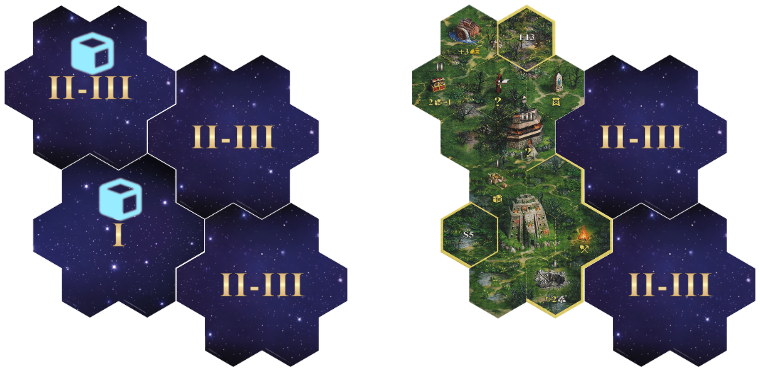
\includegraphics[width=\linewidth]{\maps/close_to_enemies_p1.png}
  \captionof{figure}{\textbf{1-PLAYER SCENARIO | EXAMPLE }}
\end{center}
\vspace*{\fill}

\end{multicols}

\begin{figure}[h!]
  \centering
  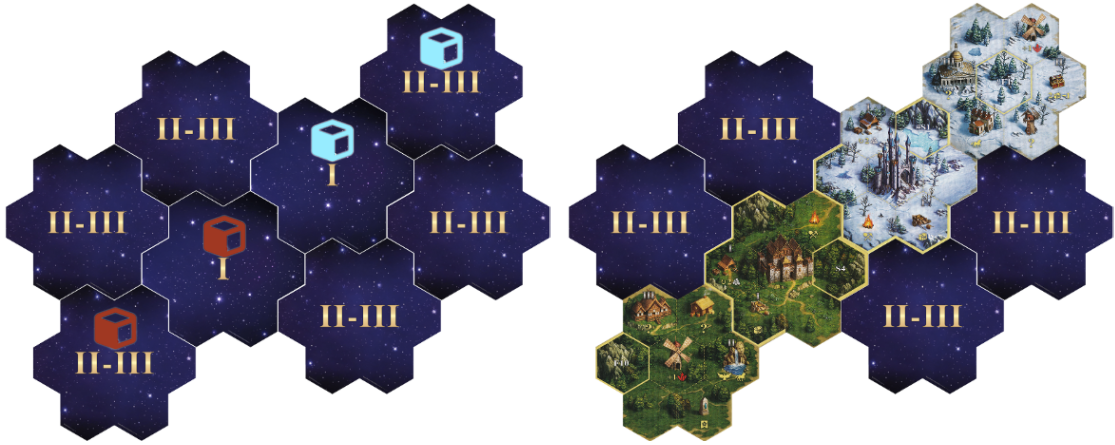
\includegraphics[width=0.75\linewidth]{\maps/close_to_enemies_p2.png}
  \captionof{figure}{\textbf{2-PLAYER SCENARIO | EXAMPLE }}
\end{figure}

\begin{table*}[b!]
  \hommtable[]{18}{
    \centering
    \medskip
    \textbf{Enemy Clan Armies}\\
    \bigskip

    \let\origbronze\bronze
    \let\origsilver\silver
    \let\origgolden\golden
    \let\origazure\azure
    \renewcommand{\bronze}{\origbronze[12]}
    \renewcommand{\silver}{\origsilver[12]}
    \renewcommand{\golden}{\origgolden[12]}
    \renewcommand{\azure}{\origazure[12]}

      \begin{tabularx}{0.95\linewidth}{p{0.2\linewidth}XXXX} &
      \darkcell{\textbf{Easy}} &
      \darkcell{\textbf{Normal}} &
      \darkcell{\textbf{Hard}} &
      \darkcell{\textbf{Impossible}}\\
      \darkcell[1.2]{First wave}
        & \lightcell[1.2]{\bronze}
        & \lightcell[1.2]{\bronze \bronze}
        & \lightcell[1.2]{\bronze \bronze \bronze}
        & \lightcell[1.2]{\bronze \bronze \silver} \\

      \darkcell[1.2]{Second wave}
        & \lightcell[1.2]{\bronze \bronze}
        & \lightcell[1.2]{\bronze \bronze \silver}
        & \lightcell[1.2]{\bronze \silver \silver}
        & \lightcell[1.2]{\silver \silver \silver} \\

      \darkcell[1.2]{Third wave}
        & \lightcell[1.2]{\bronze \silver \silver}
        & \lightcell[1.2]{\bronze \bronze \silver \silver}
        & \lightcell[1.2]{\bronze \bronze \silver \silver \silver}
        & \lightcell[1.2]{\bronze \bronze \silver \silver \golden} \\

      \darkcell[1.2]{Settlement Defenders}
        & \lightcell[1.2]{ \bronze \silver \silver \golden \golden}
        & \lightcell[1.2]{ \silver \golden \golden \golden \golden}
        & \lightcell[1.2]{ \golden \golden \golden \golden \golden}
        & \lightcell[1.2]{ \silver \golden \golden \golden \azure} \\

      \end{tabularx}
  }
\end{table*}


\begin{center}
  \vspace*{\fill}
  \begin{figure}
    \centering
    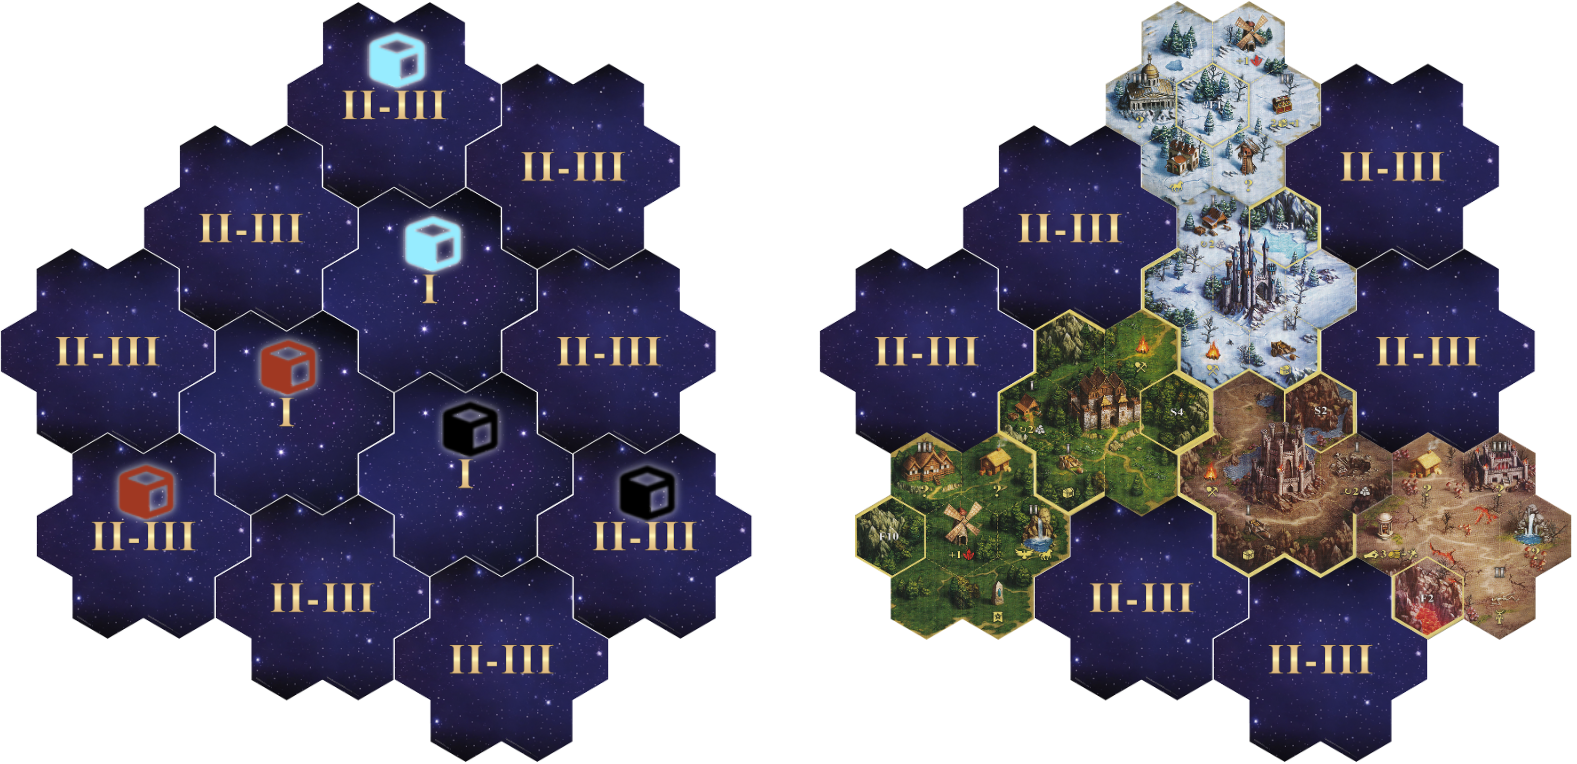
\includegraphics[width=0.75\paperwidth]{\maps/close_to_enemies_p3.png}
    \captionof{figure}{\textbf{3-PLAYER SCENARIO | EXAMPLE}}
  \end{figure}
  \vspace*{\fill}
  \begin{figure}
    \centering
    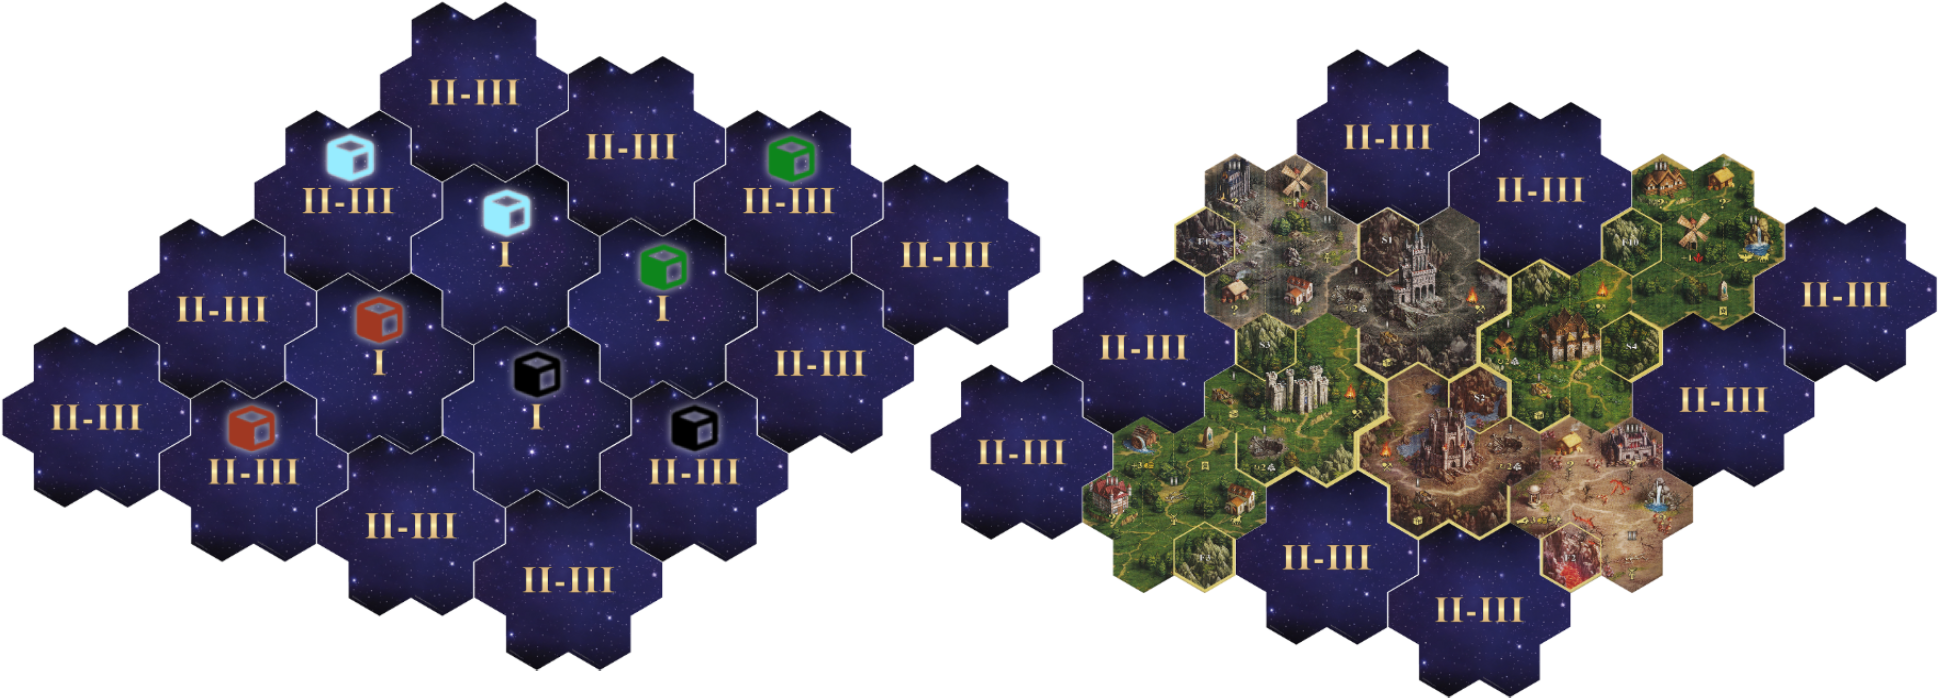
\includegraphics[width=0.85\paperwidth]{\maps/close_to_enemies_p4.png}
    \captionof{figure}{\textbf{4-PLAYER SCENARIO | EXAMPLE}}
  \end{figure}
  \vspace*{\fill}
\end{center}

\begin{tikzpicture}[overlay]
  \node(bg)[anchor=center, opacity=0.07, xshift=-2em, yshift=-24em] at (current page.south) {
    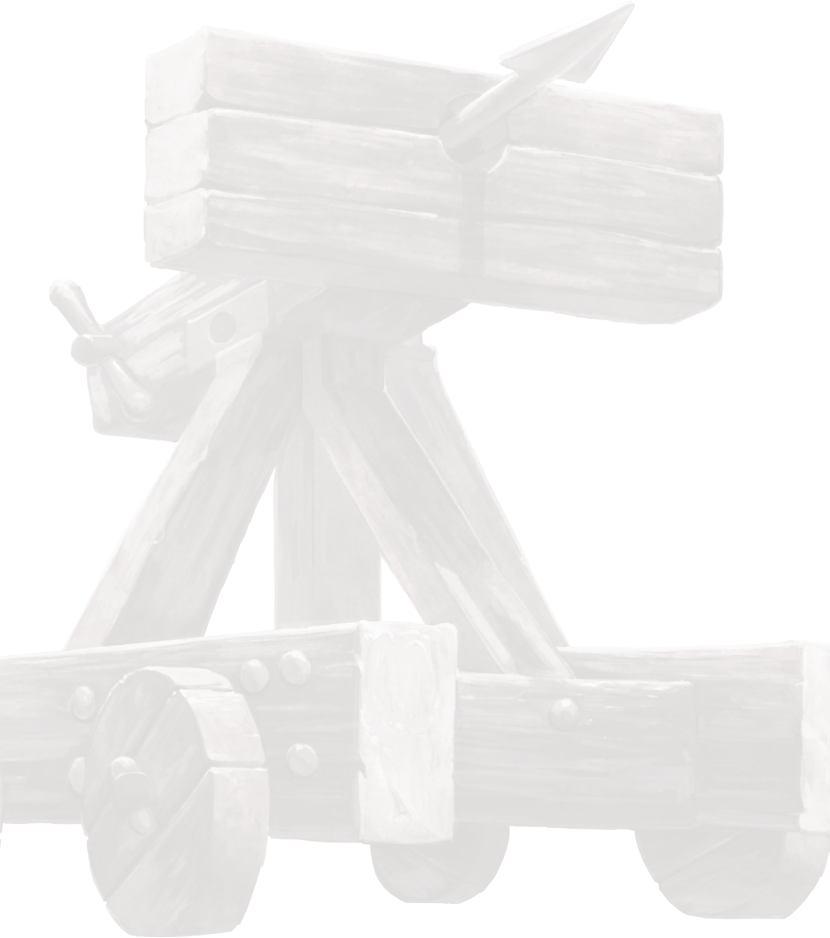
\includegraphics[width=1.1\paperwidth, keepaspectratio]{\art/ballista.png}
  };
\end{tikzpicture}
\begin{center}
  \vspace*{\fill}
  \begin{figure}[!h]
    \centering
    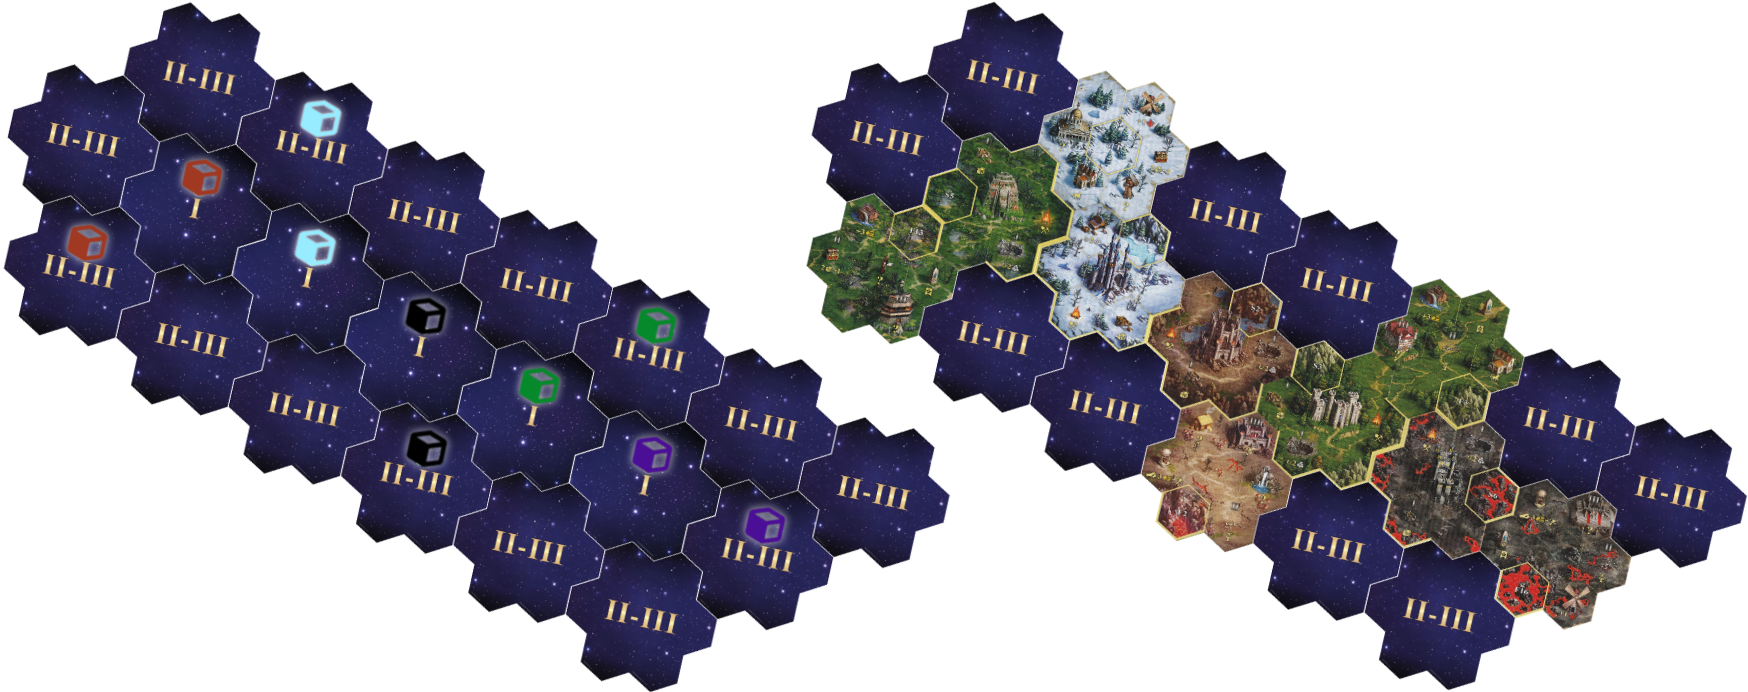
\includegraphics[width=0.75\paperwidth]{\maps/close_to_enemies_p5.png}
    \captionof{figure}{\textbf{5-PLAYER SCENARIO | EXAMPLE}}
  \end{figure}
  \vspace{5em}
  \begin{figure}[!h]
    \centering
    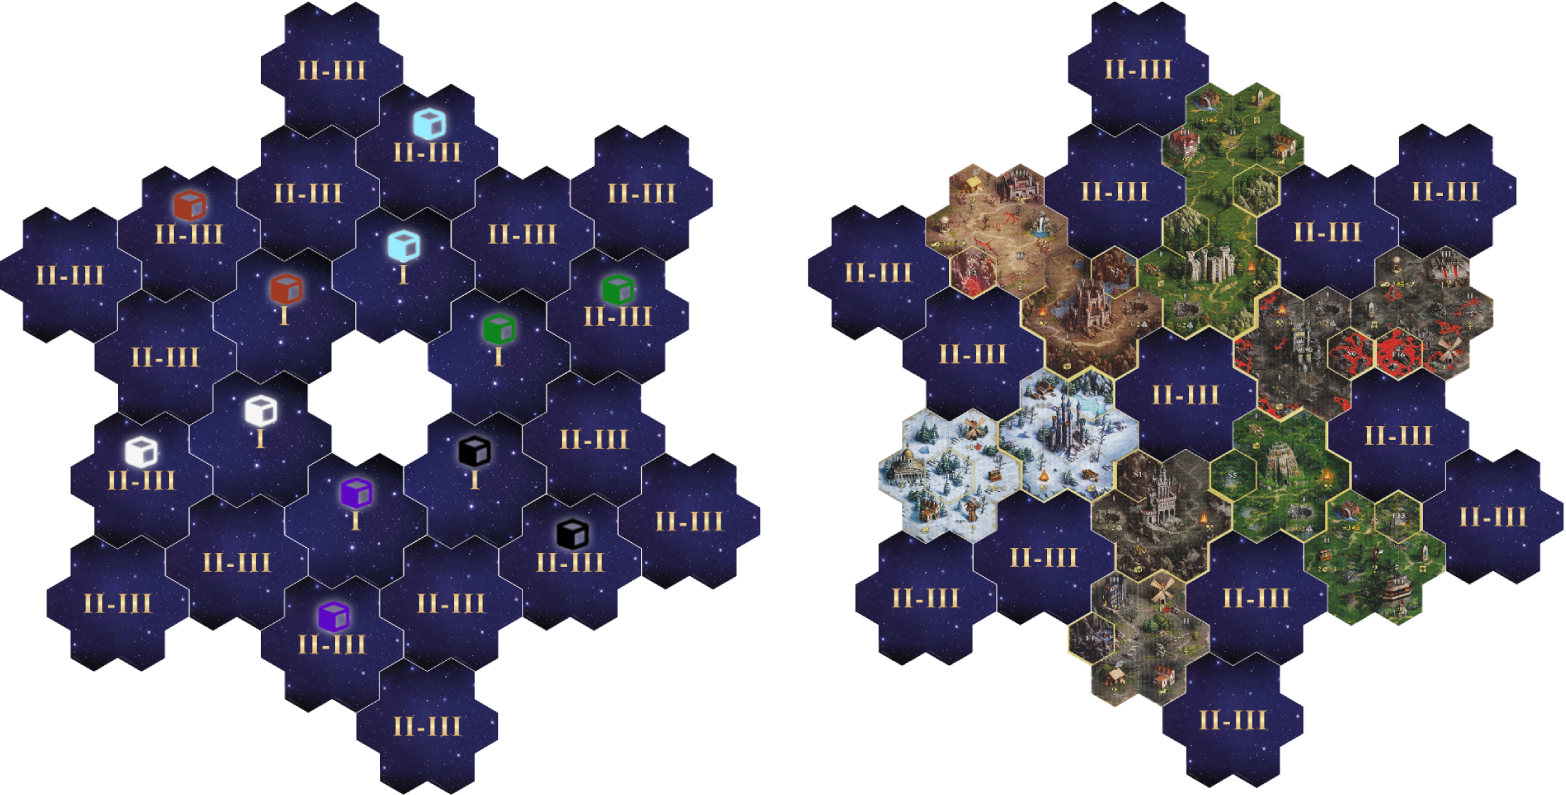
\includegraphics[width=0.75\paperwidth]{\maps/close_to_enemies_p6.png}
    \captionof{figure}{\textbf{6-PLAYER SCENARIO | EXAMPLE}}
  \end{figure}
  \vspace*{\fill}
\end{center}
